\documentclass[english,russian,a4paper,12pt]{article}
\usepackage[utf8]{inputenc}
\usepackage[T2A]{fontenc}
\usepackage{babel}
\usepackage{csquotes}

\usepackage{fullpage}
\usepackage{indentfirst}
\usepackage[font=small,labelfont=bf,labelsep=period]{caption}
\usepackage{graphicx}
\usepackage{wrapfig}
\usepackage{subcaption}
\usepackage{paralist}

\usepackage{amssymb, amsmath}

\usepackage{tikz}
\usetikzlibrary{arrows,fit,positioning,shapes.multipart}

\usepackage[
	pdfauthor={Oleg Rogozin},
	pdftitle={Convergence of new CI module},
	colorlinks,pdftex, unicode]{hyperref}

\makeatletter
\newcommand{\Rmnum}[1]{\expandafter\@slowromancap\romannumeral #1@}
\makeatother
\newcommand{\Kn}{\mathrm{Kn}}

\begin{document}

\tableofcontents

\section{Модификации метода вычисления интеграла столкновений}
В классическом проекционном методе дискретных ординат (ПМДО) [] допустимы различные вариации
алгоритма вычисления интеграла столкновения.
Ниже рассмотривается их влияние на точность аппроксимации.

\subsection{Критерий выбора узлов проецирования}

Ключевым моментом является способ отбора пары узлов проецирования \(\mathbf{p}_l,\mathbf{p}_m\) из шаблона \(\mathcal{S}\).
Консервативность ПМДО подразумевает их нахождение в противоположных сторонах от сферы радиусом \( \left|\mathbf{p}'\right| \).
Условимся считать узел \(\mathbf{p}_l\) с большей энергией:
\begin{equation}\label{eq:exist_nodes}
	\mathbf{p}_m^2 \leqslant \mathbf{p}'^2 < \mathbf{p}_l^2,
\end{equation}
тогда регуляризационный коэффициент
\begin{equation}\label{eq:r_koef}
	r = \frac{\mathbf{p}'^2-\mathbf{p}_l^2}{\mathbf{p}_m^2-\mathbf{p}_l^2}
\end{equation}
будет лежать в следующем диапазоне:
\begin{equation}\label{eq:r_criterion}
	0 < r \leqslant 1.
\end{equation}

Простейший критерий выбора заключается минимизации энергетической разницы:
\begin{equation}\label{eq:min_delta_E}
	\mathcal{L}(\mathbf{p}_{l,m}) = \left|\mathbf{p}_{l,m}^2-\mathbf{p}'^2\right| \rightarrow \min, \quad \mathbf{p}_l,\mathbf{p}_m \in \mathcal{S}.
\end{equation}
Однако в таком случае можно получить высокую ошибку аппроксимации угла разлёта (рис.~\ref{pic:r1}).

Более точный метод подразумевает сравнение импульсов.
Учитывая различный вклад каждого из узлов проецирования,
оптимальным критерием будет являться минимизация следующего функционала:
\begin{equation}\label{eq:min_delta_p}
	\mathcal{L}(\mathbf{p}_l,\mathbf{p}_m) = (1-r)(\mathbf{p}_l-\mathbf{p}')^2 + r(\mathbf{p}_m-\mathbf{p}')^2 \rightarrow \min,
	\quad \mathbf{p}_l,\mathbf{p}_m \in \mathcal{S}.
\end{equation}

\begin{figure}[ht]
		\centering
	\begin{subfigure}[b]{0.2\textwidth}
		\centering
		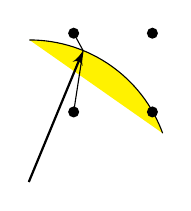
\begin{tikzpicture}[point/.style={circle, draw, fill=black, minimum size=1mm},
							>=latex', scale=1]
			\foreach \x in {20}
				\draw[fill=yellow] (1.13,-.27) arc (\x:\x+70:1.8cm);
			\foreach \x in {0,1}
				\foreach \y in {0,1}
					\fill[black] (\x,\y) circle (2pt);
			\coordinate (end) at (.12,.78);
			\draw[thick, ->] (-0.57,-0.89) -- (end);
			\draw (0,1) -- (end) -- (0,0);
		\end{tikzpicture}
		\caption{}\label{pic:r1}
	\end{subfigure}
	\begin{subfigure}[b]{0.2\textwidth}
		\centering
		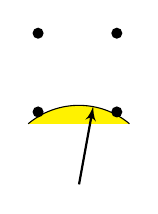
\begin{tikzpicture}[point/.style={circle, draw, fill=black, minimum size=1mm},
							>=latex', scale=1]
			\foreach \x in {130}
				\draw[fill=yellow] (-.125,-.15) arc (\x:\x-80:1cm);
			\foreach \x in {0,1}
				\foreach \y in {0,1}
					\fill[black] (\x,\y) circle (2pt);
			\draw[thick, ->] (0.52,-0.92) -- (.7,.07);
		\end{tikzpicture}
		\caption{}\label{pic:nonexist}
	\end{subfigure}
	\captionsetup{singlelinecheck=off}
	\caption[Примеры характерных случаев попадания разлётной скорости в шаблон проецирования]{
		Примеры характерных случаев попадания разлётной скорости в шаблон проецирования:
		\begin{inparaenum}[\itshape a\upshape)]
			\item высокая ошибка аппроксимации угла разлёта;
			\item не найдена соответствующая пара узлов.
		\end{inparaenum}
	}\label{fig:stencils}
\end{figure}

\subsection{Способ интегрирования по прицельному расстоянию}
Поскольку в интеграле столкновения присутствует в качестве множителя прицельное расстояние \(b\),
то можно сравнить два способа интегрирования:
\begin{equation}\label{eq:int_b}
	\int\dots bdb
\end{equation}
\begin{equation}\label{eq:int_b2}
	\int\dots db^2
\end{equation}
Во втором случае чаще будут встречаться столкновения с большим прицельным расстоянием \(b\).

\section{Соотношение различных типов точек}

Для интегрирования по 8-мерному кубу используется сетка Коробова, содержащая \(N_\mathrm{kor}\) точек.
Поскольку скоростная сетка представляет собой шар, то для численного интегрирования используется
только около четверти всех \(N_\mathrm{kor}\) узлов. Остальные просто отбрасываются.
Аналитическая оценка даёт следующее значение полезных узлов \(N_\nu\):
\[ \frac{N_\nu}{N_\mathrm{kor}} = \left(\frac{V_\mathrm{ball}}{V_\mathrm{cube}}\right) =\left(\frac\pi6\right) \approx 27.4 \%. \]

\begin{figure}[ht]
	\centering
	\includegraphics{N_nu/N_nu.pdf}
	\caption{Распределение реального количества точек интегрирования (использовано 1000 выборок).}
	\label{fig:N_nu}
\end{figure}

Здесь и далее реальные процентные значения посчитаны для следующих параметров:
\[ N_R = 26, \quad N_\Omega = 73824, \quad N_\mathrm{kor} = 2000003, \]
где \(N_R\) "--- число узлов на радиусе скоростной сетки, \(N_\Omega\) "--- полное число узлов в скоростной сетке.
Если не сказано иначе, то подразумевается метод~\eqref{eq:min_delta_p} и~\eqref{eq:int_b}.

В зависимости от случайного вектора сдвига сетки Коробова реальное значение \(N_\nu/N_\mathrm{kor}\)
колеблется в диапазоне \(27.4\% \div 27.7\%\). Среднее значение 27.57\%.
Гистограмма этого распределения представлена на рис.~\ref{fig:N_nu}.

Из общего числа \(N_\nu\) можно выделить несколько специальных классов точек,
для которых метод рассчёта столкновений отличается от основного.
Таких точек достаточно много (37.5\%).

\renewcommand{\labelenumi}{\Roman{enumi}.}
\renewcommand{\labelenumii}{\arabic{enumii}}
\begin{enumerate}
	\item 28.4\% столкновений происходят так, что функция распределения не претерпевает изменений.
	Это возможно в трёх различных ситуациях.
	\begin{enumerate}
		\item Если разлётные скорости выходят за пределы скоростного пространства \(\Omega_R\).
		Число таких точек равно 25.2\%.
		
		\item Если разлётная скорость оказалась внутри \(\Omega_R\),
		но одна из используемых точек шаблона проецирования вышла за пределы \(\Omega_R\).
		Доля таких столкновений составляет 3.1\%.
		
		\item При малом угле разлёта одна из \(\mathbf{p}_{l,m}\) может совпадать
		с начальной скоростью \(\mathbf{p}\). Вероятность такого события порядка 0.08\%.
	\end{enumerate}

	\item На восьмиточечном шаблоне может возникнуть такая ситуация,
	что пара проекционных узлов, удовлетворяющих~\eqref{eq:exist_nodes} не будет найдена (рис.~\ref{pic:nonexist}).
	Это означает, что в шаблоне не оказалось точек с меньшей энергией, чем разлётная.
	Количество такого рода особых точек мало (0.01\%), поэтому их можно просто исключить из \(N_\nu\).
	Более прецизионной альтернативой является расширение шаблона до 32 точек специально для этого случая.

	\item Наконец, в 9.2\% случаев регуляризационный коэффициент принимает крайнее значение \(r=1\).
	Тогда расчёт соответствующего столкновения значительно упрощается,
	поскольку отпадает необходимость в процедуре проецирования.
\end{enumerate}

\subsection{Критерий выбора узлов проецирования}

В зависимости от выбранного критерия выбора исследуемое соотношение между специальными классами точек
претерпевает изменения. Наиболее ярко они выражены для последнего типа точек.
Использование критерия~\eqref{eq:min_delta_E} увеличивает количество узлов \Rmnum{3} рода до 22.4\%,
что, как было указано выше, создаёт б\'{о}льшую невязку аппроксимации.
Из тех же соображений количество \Rmnum{1}.3 также возрастает до 0.2\%.

\subsection{Способ интегрирования по прицельному расстоянию}

При переходе к интегрированию по квадрату прицельного расстояния \(b\)
удвается число точек \Rmnum{1}.3, в которых отклонения траектории не происходит.
Кроме того, увеличивается процент \Rmnum{1}.1 до 28.9\%.

Можно предположить, что больший вклад результирующий интеграл столкновений вносят узлы с небольшими \(b\),
поскольку именно такие столкновения более всего перемешивают газ.
Поэтому предпочтительно использовать равномерный способ~\eqref{eq:int_b}.
Однако при исследовании эффектов, зависящих больше от высокоскоростных молекул (например, в ударной волне),
может дать преимущества метод~\eqref{eq:int_b2}.

\section{Сходимость различных модификаций}

Анализируется одномерная задача переноса тепла между двумя плоскими параллельными пластинами.
Исследуется сходимость коэффициента теплопроводности \(\lambda\) для газа, состоящего из твёрдых сфер, к эталонному
\[ \lambda_\mathrm{ref} = 2.129475. \]

\begin{figure}[ht]
	\centering
	\includegraphics{heat_radius/convergence.pdf}
	\caption{Отклонение коэффициента теплопроводности \(\lambda\) от эталонного \(\lambda_\mathrm{ref}\)
		в зависимости от числа узлов на радиусе скоростной сетки \(N_R\).}
	\label{fig:heat_radius}
\end{figure}

Задача моделировалась для \(\xi_{cut} = 4.3 \sqrt{2RT}\) при различных объёмах скоростной сетки и сетки Коробова.
Разница температур на стенках достаточно мала, чтобы считать задачу линейной:
\[ \frac{\Delta T}{T} = 0.01. \]
В физическом одномерном пространстве имеется \(N_x=40\) ячеек, длиной \(h=0.5\), так что число Кнудсена \(\Kn=0.05\).
Для повышения точности проводится процедура усреднения по ряду временн\'{ы}х значений в стационарном режиме.

\begin{figure}[ht]
	\centering
	\includegraphics{heat_korobov/convergence.pdf}
	\caption{Отклонение коэффициента теплопроводности \(\lambda\) от эталонного \(\lambda_\mathrm{ref}\)
		в зависимости от мощности сетки Коробова \(N_\mathrm{kor}\).}
	\label{fig:heat_korobov}
\end{figure}

\begin{figure}[ht]
	\centering
	\includegraphics{heat_korobov/korobov.pdf}
	\caption{Среднеквадратичное отклонение коэффициента теплопроводности \(\lambda\) во времени
		в зависимости от мощности сетки Коробова \(N_\mathrm{kor}\).}
	\label{fig:var_korobov}
\end{figure}

Результаты моделирования представлены на рис.~\ref{fig:heat_radius} и~\ref{fig:heat_korobov}.

Синим цветом на рис.~\ref{fig:heat_radius} показаны значения для старого модуля интеграла столкновений,
на которых чётко наблюдается второй порядок сходимости по \(N_R\).
Видно, что любая модификация нового модуля имеет меньшую невязку,
однако для больших \(N_R\) наблюдается в целом неопределённое поведение.

В любом случае стоит предпочесть метод~\eqref{eq:min_delta_p} и~\eqref{eq:int_b} (показан зелёным цветом),
поскольку он обеспечивает как меньшую невязку аппроксимации, так и более стабильную сходимость для больших \(N_R\).

Особенно чётко флуктуационный характер сходимости виден на рис.~\ref{fig:heat_korobov}.
Можно констатировать, что от мощности сетки Коробова \(N_\mathrm{kor}\) точность результата
практически не зависит.

Кроме того, из рис.~\ref{fig:var_korobov} видно, что увеличение мощности сетки Коробова выше \(10^6\)
не уменьшает временн\'{ы}е колебания измеряемого коэффициента теплопроводности,
так что среднеквадратичное отклонение \(\sigma(\lambda)\) не опускается ниже значения 0.005.

\section{Заключение}

\begin{enumerate}
	\item Рассмотрены все возможные специфические случаи столкновений.
	\item Показана большая точность критерия отбора проекционных узлов~\eqref{eq:min_delta_p}.
	\item Исследовано влияние мощности сетки Коробова \(N_\mathrm{kor}\) на точность моделирования.
	\item До сих пор не выявлены различия, обуславливающие значительное несовпадение результатов расчётов с помощью
	нового и старого модулей интеграла столкновения.
	\item Выдвинуто предположение, что <<узким горлышком>> точности программной среды является
	приближённое вычисление операции возведения в степень при регуляризации функции распределения
	между узлами проецирования.
\end{enumerate}

\end{document}


